% Begin the document and set up the style of the document
\documentclass[a4paper,11pt]{article}

% Install the required packages for the document 
\usepackage{enumitem}
\usepackage{amsmath}
\usepackage{amssymb}
\usepackage{verbatim}
\usepackage{mathtools}
\usepackage{tikz}
\usepackage{nicefrac}
\usepackage{bm}

\newcommand{\norm}[1]{\left\lVert#1\right\rVert}


% Page and style settings
%\parskip=8pt
\parindent=0pt
% Right margin
\textwidth=6.25in
% Left margin
\oddsidemargin=0pt
\evensidemargin=0pt
% Bottom margin
\textheight=10in
% Top margin
\topmargin=-0.75in
\baselineskip=11pt
% end of page and other style settings

\renewcommand{\familydefault}{\sfdefault}
\usepackage{calrsfs}
\DeclareMathAlphabet{\pazocal}{OMS}{zplm}{m}{n}

\newcommand{\indep}{\mathrel{\text{\scalebox{1.07}{$\perp\mkern-10mu\perp$}}}}
\newcommand{\p}{\mathbb{P}}
\newcommand{\e}{\mathbb{E}}
\newcommand{\ds}{\displaystyle}
\newcommand{\code}{\texttt}
\newcommand{\HRule}{\rule{\linewidth}{0.5mm}} % Defines a new command for the horizontal lines, change thickness here

\newenvironment{nscentre}
 {\parskip=0pt\par\nopagebreak\centering}
 {\par\noindent\ignorespacesafterend}


\usepackage{fullpage}

\usepackage{titlesec} % Used to customize the \section command
\titleformat{\section}{\bf}{}{0em}{}[\titlerule] % Text formatting of sections
\titlespacing*{\section}{0pt}{3pt}{3pt} % Spacing around sections

\begin{document}
\setlength{\abovedisplayskip}{8pt}{%
\setlength{\belowdisplayskip}{8pt}{%


\text{School of Mathematics}
\hfill
\text{University of New South Wales}

\begin{nscentre}
	\textbf{MATH2701: Abstract Algebra and Fundamental Analysis}\\
	\textbf{Short Assignment 2}\\
\end{nscentre}

\text{Name: Keegan Gyoery}
\hfill
\text{zID: z5197058}

\pagenumbering{arabic}
	\begin{enumerate}[leftmargin=*]
		\item Firstly, we must generalise Young's Inequality, using Jensen's Inequality. Suppose that $\ds{f:R \rightarrow R}$ is convex, that $\ds{x_1,\dots, x_n \in \mathbb{R}}$ and $\ds{a_1,\dots, a_n > 0}$. Then
			\begin{align*}
				f\left(\frac{\sum a_ix_i}{\sum a_j}\right) & \leq \frac{\sum a_if(x_i)}{\sum a_j}.
			\end{align*}
			Let $\ds{\lambda_i = \frac{a_i}{\sum a_j}}$, and consider $\ds{f(x) = -\ln{x}}$, which is convex. Furthermore, from the question, we have
			\begin{align*}
				\sum_{l=1}^k \frac{1}{p_l} & = 1.
			\end{align*}
			Now, taking $\ds{\lambda_i = \frac{1}{p_i}}$, and suppose $\ds{c_1,\dots,c_n > 0}$. Letting $\ds{x_i = c_i^{p_i}}$, by Jensen's Inequality, we have
			\begin{align*}
				-\ln\left(\frac{c_1^{p_1}}{p_1} + \frac{c_2^{p_2}}{p_2} + \dots + \frac{c_n^{p_n}}{p_n}\right) & \leq -\frac{1}{p_1}\ln{c_1^{p_1}} - \frac{1}{p_2}\ln{c_2^{p_2}}- \dots -\frac{1}{p_n}\ln{c_n^{p_n}}\\
																											   & = -\ln(c_1c_2\dots c_n).
			\end{align*}
			Exponentiating gives the inequality 
			\begin{align*}
				c_1c_2\dots c_n & \leq \frac{c_1^{p_1}}{p_1} + \frac{c_2^{p_2}}{p_2} + \dots + \frac{c_n^{p_n}}{p_n} \dots (1).
			\end{align*}
			Using the triangle inequality,
			\begin{align*}
				\left| \sum_{i=1}^n x_{1,i}x_{2,i}\dots x_{k,i} \right| & \leq \sum_{i=1}^n |x_{1,i}||x_{2,i}|\dots |x_{k,i}|,
			\end{align*}
			and so it suffices to prove the result in the case that all the numbers are non-negative. We may assume that all the $\ds{x_{j,i}}$ are strictly positive since if $\ds{x_{j,i} = 0}$, then omitting the $\ds{i}$-th terms of the sums doesn’t change the left-hand side of the required result, and can only make the right-hand side of the required result smaller. Now, setting
			\begin{align*}
				A_1 & = c_1^{p_1}, A_2 = c_2^{p_2}, \dots , A_k = c_k^{p_k},
			\end{align*}
			and considering the inequality given by $\ds{(1)}$, we have 
			\begin{align*}
				A_1^{\nicefrac{1}{p_1}}A_2^{\nicefrac{1}{p_2}}\dots A_k^{\nicefrac{1}{p_k}} & \leq \frac{1}{p_1}A_1 + \frac{1}{p_2}A_2 + \dots + \frac{1}{p_k}A_k \dots (2).
			\end{align*}
			For ease of notation, let 
			\begin{align*}
				X_1 & = \sum_{i=1}^nx_{1,i}^{p_1}, X_2 = \sum_{i=1}^nx_{2,i}^{p_2}, \dots , X_k = \sum_{i=1}^nx_{k,i}^{p_k},
			\end{align*}
			and furthermore, for $\ds{i = 1,\dots,n}$, let
			\begin{align*}
				A_{1,i} & = \frac{x_{1,i}^{p_1}}{X_1}, A_{2,i} = \frac{x_{2,i}^{p_2}}{X_2}, \dots , A_{k,i} = \frac{x_{k,i}^{p_k}}{X_k},
			\end{align*}
			so that,
			\begin{align*}
				\sum_{i=1}^nA_{1,i} & = \sum_{i=1}^nA_{2,i} = \dots = \sum_{i=1}^nA_{k,i} = 1.
			\end{align*}
			Using the above result $\ds{(2)}$, we have
			\begin{align*}
				\sum_{i=1}^n x_{1,i}x_{2,i}\dots x_{k,i} & = \sum_{i=1}^nX_1^{\nicefrac{1}{p_1}}A_{1,i}^{\nicefrac{1}{p_1}}X_2^{\nicefrac{1}{p_2}}A_{2,i}^{\nicefrac{1}{p_2}}\dots X_k^{\nicefrac{1}{p_k}}A_{k,i}^{\nicefrac{1}{p_k}}\\
														 & = X_1^{\nicefrac{1}{p_1}}X_2^{\nicefrac{1}{p_2}}\dots X_k^{\nicefrac{1}{p_k}} \sum_{i=1}^nA_{1,i}^{\nicefrac{1}{p_1}}A_{2,i}^{\nicefrac{1}{p_2}}\dots A_{k,i}^{\nicefrac{1}{p_k}}\\
														 & \leq \prod_{l=1}^k X_l^{\nicefrac{1}{p_l}} \left[\frac{1}{p_1} \sum_{i=1}^n A_{1,i} + \frac{1}{p_2} \sum_{i=1}^n A_{2,i} + \dots + \frac{1}{p_k} \sum_{i=1}^n A_{k,i}\right]\\
														 & = \prod_{l=1}^k X_l^{\nicefrac{1}{p_l}} \left[\frac{1}{p_1} + \frac{1}{p_2} + \dots + \frac{1}{p_k} \right]\\
														 & = \prod_{l=1}^k X_l^{\nicefrac{1}{p_l}}\\
														 & = \prod_{l=1}^k \left(\sum_{i=1}^nx_{l,i} \right)^{\nicefrac{1}{p_l}}\\
														 & = \prod_{l=1}^k \left\lVert{\bm{x}_l}\right\rVert _{p_l}\\
				\therefore \sum_{i=1}^n x_{1,i}x_{2,i}\dots x_{k,i} & \leq \prod_{l=1}^k \left\lVert{\bm{x}_l}\right\rVert _{p_l}
			\end{align*}

		\item 
			\begin{enumerate}
				\item Given orthonormal vectors $\ds{\bm{x}_1, \bm{x}_2,\dots, \bm{x}_n}$ and $\ds{d_1, d_2, \dots , d_n}$ positive numbers, we have the set,
					\begin{align*}
						E & = \left\{ \bm{x} = \sum_{k = 1}^n c_k \bm{x}_k : \frac{c_1^2}{d_1^2} + \frac{c_2^2}{d_2^2} + \dots + \frac{c_n^2}{d_n^2} \leq 1 \right\}.
					\end{align*}
					To prove that ellipsoids are convex bodies, we must prove that $\ds{E}$ is a non-empty subset of $\ds{\mathbb{R}^n}$, convex, centrally symmetric, closed, and bounded above and below. Firstly, for convexity of $\ds{E}$, consider two vectors $\ds{\bm{x}, \bm{y} \in E}$ where,
					\begin{align*}
						\bm{x} & = \sum_{k = 1}^n a_k \bm{x}_k \text{ and } \bm{y} = \sum_{k = 1}^n b_k \bm{x}_k.
					\end{align*}
					For later use, we will label the following vectors,
					\begin{align*}
						\bm{a} & = \left(\frac{a_1}{d_1}, \frac{a_2}{d_2}, ... , \frac{a_n}{d_n}\right) \text{ and } \bm{b} = \left(\frac{b_1}{d_1}, \frac{b_2}{d_n}, ... , \frac{b_n}{d_n}\right).
					\end{align*}
					Given $\ds{\bm{x}, \bm{y} \in E}$, we have $\ds{\bm{a} \cdot \bm{a} = \norm{\bm{a}}^2 \leq 1}$ and $\ds{\bm{b} \cdot \bm{b} = \norm{\bm{b}}^2 \leq 1.}$
					Now, consider the vector $\ds{\bm{w} = \lambda \bm{x} + (1 - \lambda) \bm{y}}$ for any $\ds{\lambda \in [0,1]}$. As a result, we have,
					\begin{align*}
						\bm{w} & = \sum_{k = 1}^n (\lambda a_k + (1 - \lambda) b_k)\bm{x_k}.
					\end{align*}
					Let $\ds{v_k = (\lambda a_k + (1 - \lambda) b_k)}$. We can thus rewrite $\ds{\bm{w} = \sum_{k = 1}^n v_k\bm{x_k}}$. Consider the following,
					\begin{align*}
						\frac{v_1^2}{d_1^2} + \frac{v_2^2}{d_2^2} + ... + \frac{v_n^2}{d_n^2} & = \sum_{k = 1}^n \frac{(\lambda a_k + (1 - \lambda) b_k)^2}{d_k^2} \\
			& = \sum_{k = 1}^n \left(\lambda^2 \frac{a_k^2}{d_k^2} + (1 - \lambda)^2 \frac{b_k^2}{d_k^2} + 2\lambda(1 - \lambda) \frac{a_kb_k}{d_k^2}\right) \\
			& = \lambda^2 (\bm{a} \cdot \bm{a}) + (1 - \lambda)^2 (\bm{b} \cdot \bm{b}) + 2\lambda(1 - \lambda) (\bm{a} \cdot \bm{b}) \\
			& \leq \lambda^2 + (1 - \lambda)^2 + 2\lambda(1 - \lambda) \norm{\bm{a}} \norm{\bm{b}} \hspace{5mm} \text{by Cauchy-Schwarz} \\
			& \leq \lambda^2 + (1 - \lambda)^2 + 2\lambda(1 - \lambda) \\
			& = 1
					\end{align*}
					Hence $\ds{\bm{w} \in E}$, and thus ellipsoids are convex.
					Now, for centrally symmetric, we consider $\ds{\bm{x} \in E}$, such that
					\begin{align*}
						\bm{x} & = \sum_{k = 1}^n c_k \bm{x}_k \text{ and } \frac{c_1^2}{d_1^2} + \frac{c_2^2}{d_2^2} + \dots + \frac{c_n^2}{d_n^2} \leq 1.
					\end{align*}
					Considering $\ds{-\bm{x}}$, 
					\begin{align*}
						-\bm{x} & = \sum_{k = 1}^n (-c_k) \bm{x}_k\\
						\therefore \frac{(-c_1)^2}{d_1^2} + \frac{(-c_2)^2}{d_2^2} + \dots + \frac{(-c_n)^2}{d_n^2} & = \frac{c_1^2}{d_1^2} + \frac{c_2^2}{d_2^2} + \dots + \frac{c_n^2}{d_n^2} \leq 1\\
				  \therefore \frac{(-c_1)^2}{d_1^2} + \frac{(-c_2)^2}{d_2^2} + \dots + \frac{(-c_n)^2}{d_n^2} & \leq 1.\\
					\end{align*}
					Clearly, $\ds{-\bm{x} \in E}$, and so $\ds{E}$ is centrally symmetric. We also know that $\ds{E}$ contains its boundary. The boundary is given by,
					\begin{align*}
						\partial E & = \left\{ \bm{x} = \sum_{k = 1}^n c_k \bm{x_k} : \frac{c_1^2}{d_1^2} + \frac{c_2^2}{d_2^2} + \dots + \frac{c_n^2}{d_n^2} = 1 \right\},
					\end{align*}
					which is clearly a subset of $\ds{E}$. Hence $\ds{E}$ is closed. Finally we also know that $\ds{E}$ is bounded above and below. Specifically it is bounded above by the ball $\ds{B_D}$ where $\ds{D = \max\{d_k\}}$. To check, consider $\ds{\bm{x} \in E}$ where $\ds{\norm{\bm{x}} > D}$. Then we have
					\begin{align*}
						c_1^2 + \dots + c_n^2 & > D^2 \\
						\frac{c_1^2}{D^2} + \dots + \frac{c_n^2}{D^2} & > 1.
					\end{align*}
					But we also have,
					\begin{align*}
						\frac{c_1^2}{D^2} + \dots+ \frac{c_n^2}{D^2} & \leq \frac{c_1^2}{d_1^2} + ... + \frac{c_n^2}{d_n^2} \leq 1.
					\end{align*}
					By contradiction, no such $\ds{\bm{x}}$ exists and hence $\ds{E}$ is bounded above by the ball $\ds{B_D}$. Thus, all ellipsoids are convex bodies.


				\item Let $\ds{\bm{y} = \sum_{k = 1}^n a_k\bm{x_k}}$ and consider $\ds{\bm{x} \cdot \bm{y} \leq 1}$ for all $\ds{\bm{x} = \sum_{k = 1}^n c_k \bm{x_k} \in E}$.
					\begin{align*}
						\bm{x} \cdot \bm{y} & = \sum_{k = 1}^n a_kc_k \\
						& = \sum_{k = 1}^n (d_ka_k)\left(\frac{c_k}{d_k}\right) \\
						& \leq \left(\sum_{k = 1}^n (d_ka_k)^2\right)^{\frac{1}{2}} \left(\sum_{k = 1}^n \left(\frac{c_k}{d_k}\right)^2\right)^\frac{1}{2} \hspace{5mm} \text{by Cauchy-Schwarz} \\
						& \leq \left(\sum_{k = 1}^n d_k^2a_k^2\right)^{\frac{1}{2}}
					\end{align*}
					Considering the condition for equality in Cauchy-Schwarz, we have,
					\begin{align*}
						K^{\circ} & = \left\{ \bm{y} = \sum_{k = 1}^n a_k \bm{x_k} : \frac{a_1^2}{d_1^{-2}} + \frac{a_2^2}{d_2^{-2}} + ... + \frac{a_n^2}{d_n^{-2}} \leq 1 \right\},
					\end{align*}
					which is an ellipsoid with corresponding set of positive numbers $\ds{d_1^{-1}, d_2^{-1}, ..., d_n^{-1}}$.
	
		\end{enumerate}

	\item
		The set, $\ds{K = \{(x,y) \in \mathbb{R}^2 : \max\{|x - y|, |x|, |y|\} \leq 1\}}$
		is indicated in the following diagram.

		\begin{center}
		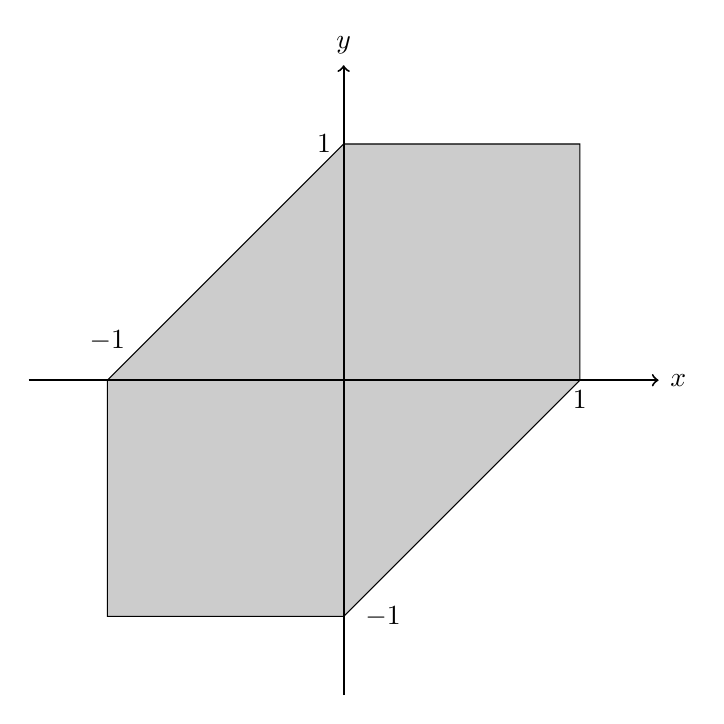
\begin{tikzpicture}
			\draw [fill=black!20!white] (-3,0)--(0,3)--(3,3)--(3,0)--(0,-3)--(-3,-3)--cycle;
			\draw [->][line width=0.25mm] (-4,0) -- (4,0);
			\draw [->][line width=0.25mm] (0,-4) -- (0,4);

			\node at (4.25, 0) {$x$};
			\node at (0, 4.25) {$y$};
			\node at (-0.25, 3) {$1$};
			\node at (3, -0.25) {$1$};
			\node at (0.5, -3) {$-1$};
			\node at (-3, 0.5) {$-1$};

		\end{tikzpicture}
		\end{center}
		\pagebreak
		Consider $\ds{\bm{u} = (x_1, y_1) \in K}$ and $\ds{\bm{v} = (x_2, y_2) \in \mathbb{R}^2}$, where $\ds{\bm{u} \cdot \bm{v} \leq 1 \implies x_1x_2 + y_1y_2 \leq 1}$. Considering the diagram below, it is obvious that for $\ds{\bm{u}, \bm{v}}$ in the light-grey shaded region, $\ds{\bm{u}\cdot \bm{v} \leq 1}$. However, as $\ds{\bm{u}}$ can also reside in the dark-grey shaded regions, $\ds{\bm{v}}$ cannot, as otherwise $\ds{\bm{u} \cdot \bm{v} > 1}$. So, by symmetry, $\ds{\bm{v}}$ can also reside in the black shaded regions, as $\ds{\bm{u}}$ cannot. 
		\begin{center}
		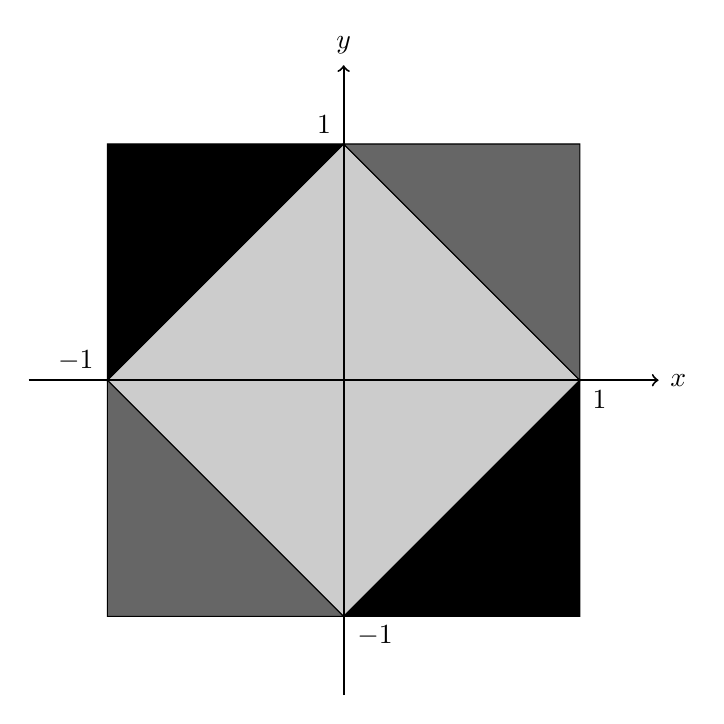
\begin{tikzpicture}
			\draw [fill=black!20!white] (-3,0)--(0,3)--(3,0)--(0,-3)--cycle;
			\draw [fill=black!60!white] (-3,0)--(-3,-3)--(0,-3)--cycle;
			\draw [fill=black!60!white] (3,0)--(3,3)--(0,3)--cycle;
			\draw [fill=black!100!white] (-3,0)--(-3,3)--(0,3)--cycle;
			\draw [fill=black!100!white] (3,0)--(3,-3)--(0,-3)--cycle;
			\draw [->][line width=0.25mm] (-4,0) -- (4,0);
			\draw [->][line width=0.25mm] (0,-4) -- (0,4);

			\node at (4.25, 0) {$x$};
			\node at (0, 4.25) {$y$};
			\node at (-0.25, 3.25) {$1$};
			\node at (3.25, -0.25) {$1$};
			\node at (0.4, -3.25) {$-1$};
			\node at (-3.4, 0.25) {$-1$};

		\end{tikzpicture}
		\end{center}
		Hence we can write,
		$$K^{\circ} = \{(x,y) \in \mathbb{R}^2 : \max\{|x + y|, |x|, |y|\} \leq 1\}.$$
		This is simply a rotation of $K$, with boundary as shown below.

		\begin{center}
		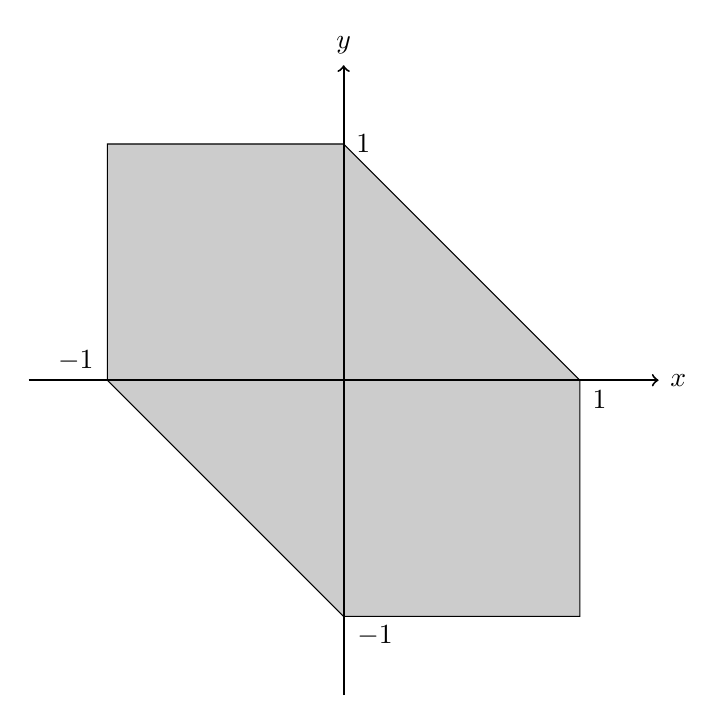
\begin{tikzpicture}
			\draw [fill=black!20!white] (-3,0)--(0,-3)--(3,-3)--(3,0)--(0,3)--(-3,3)--cycle;
			\draw [->][line width=0.25mm] (-4,0) -- (4,0);
			\draw [->][line width=0.25mm] (0,-4) -- (0,4);

			\node at (4.25, 0) {$x$};
			\node at (0, 4.25) {$y$};
			\node at (0.25, 3) {$1$};
			\node at (3.25, -0.25) {$1$};
			\node at (0.4, -3.25) {$-1$};
			\node at (-3.4, 0.25) {$-1$};

		\end{tikzpicture}
		\end{center}

		Now we can compute the Mahler volume,
		$$M(K) = \text{vol}(K) \text{vol}(K^{\circ}) = 3 \times 3 = 9.$$
	\item
		\begin{enumerate}
			\item First note that if $\ds{M = \max_{a \leq x \leq b} |f(x)|}$, then we also have $\ds{M^p = \max_{a \leq x \leq b} |f(x)|^p}$. Therefore,
			\begin{align*}
				\norm{f}_p & = \left(\int_a^b |f(x)|^p dx\right)^{\frac{1}{p}} \\
				& \leq \left(M^p \int_a^b dx\right)^{\frac{1}{p}} \\
				& = M(b - a)^{\frac{1}{p}}.
			\end{align*}
			This gives us the right hand side of the inequality,
			\begin{align*}
				\norm{f}_p \leq (b - a)^{\frac{1}{p}}M.
			\end{align*}

			\item Taking the limit of the inequality in part (a),
			\begin{align*}
				\lim_{p \rightarrow \infty} c^{\frac{1}{p}} (M - \varepsilon) \leq & \lim_{p \rightarrow \infty} \norm{f}_p \leq \lim_{p \rightarrow \infty} (b - a)^{\frac{1}{p}} M \\
				M - \varepsilon \leq & \lim_{p \rightarrow \infty} \norm{f}_p \leq M \\
				- \varepsilon \leq & \lim_{p \rightarrow \infty} \norm{f}_p - M \leq 0 \\
				& \left|\lim_{p \rightarrow \infty} \norm{f}_p - M\right| \leq \varepsilon
			\end{align*}
			Suppose $\ds{\left|\lim_{p \rightarrow \infty} \norm{f}_p - M\right| = k \neq 0}$. Then consider $\ds{\varepsilon = \frac{k}{2} < k}$. This contradicts the inequality above, and hence by contradiction, $\ds{\left|\lim_{p \rightarrow \infty} \norm{f}_p - M\right| = 0}$.
			\begin{align*}
				\therefore \lim_{p \rightarrow \infty} \norm{f}_p = M.
			\end{align*}
			\end{enumerate}

	\end{enumerate}
\end{document}
